\documentclass[UTF8,11pt,a4paper]{ctexart}

\usepackage[a4paper,top=2.35cm,bottom=2.35cm,left=2.55cm,right=2.55cm]{geometry}
\usepackage{amsmath,amssymb,bm}
\usepackage{booktabs,tabularx,longtable,array,multirow}
\usepackage{graphicx,float,subcaption}
\usepackage{xcolor}
\usepackage{fancyhdr}
\usepackage{enumitem}
\usepackage{hyperref}
\usepackage{microtype}

\definecolor{accent}{HTML}{355070}
\definecolor{accenttwo}{HTML}{2A9D8F}
\definecolor{softgray}{HTML}{F3F5F7}
\hypersetup{colorlinks=true,linkcolor=accent,citecolor=accent,urlcolor=accenttwo}
\setlength{\parindent}{2em}
\setlength{\parskip}{0.18em}
\setlist{nosep,leftmargin=2.2em}
\captionsetup{font=small,labelfont=bf}

\pagestyle{fancy}
\setlength{\headheight}{14pt}
\fancyhf{}
\fancyhead[L]{共享单车需求统计建模}
\fancyhead[R]{六专家自适应融合框架}
\fancyfoot[C]{\thepage}
\renewcommand{\headrulewidth}{0.4pt}

\newcommand{\Eone}{\textnormal{E1}}
\newcommand{\Etwo}{\textnormal{E2}}
\newcommand{\Ethree}{\textnormal{E3}}
\newcommand{\Efour}{\textnormal{E4}}
\newcommand{\Efive}{\textnormal{E5}}
\newcommand{\Esix}{\textnormal{E6}}

\begin{document}
\hypersetup{pageanchor=false}

\begin{titlepage}
  \thispagestyle{empty}
  \centering
  \vspace*{1.6cm}
  {\zihao{2}\bfseries 统计模型与 Python 实践课程项目\par}
  \vspace{2.2cm}
  {\zihao{-1}\bfseries 面向天气冲击与恢复过程的\par}
  \vspace{0.45cm}
  {\zihao{-1}\bfseries 多专家自适应共享单车需求预测\par}
  \vspace{0.9cm}
  
  \vfill
  \begin{tabular}{rl}
    姓名：& \rule{7cm}{0.4pt}\\[0.7em]
    学号：& \rule{7cm}{0.4pt}\\[0.7em]
    班级：& \rule{7cm}{0.4pt}\\[0.7em]
    指导教师：& \rule{7cm}{0.4pt}
  \end{tabular}
  \vfill
  {\zihao{-4}2026 年 9 月 10 日\par}
\end{titlepage}

\pagenumbering{Roman}
\hypersetup{pageanchor=true}

\begin{abstract}
共享单车需求与当前天气及此前一段时间的天气过程共同相关。即使当前均无雨，持续干燥与降雨刚结束也可能对应不同的出行需求。本文以这一现象为切入点，将天气历史及恢复过程纳入短期需求预测，并提出“专而治之”的六专家框架。需求、天气和恢复专家分别刻画需求惯性、当前天气响应与降雨历史，时序卷积网络（TCN）、门控循环单元（GRU）和轻量 Transformer 分别学习局部模式、递归记忆与跨日依赖。各专家采用不同的输入组织与模型结构，独立预测未来 $h\in\{1,2,3,6\}$ 小时的完整需求，再由低维状态融合层联合拟合预测权重。框架以专门化分工控制各学习器的规模，以自适应组合发挥统计模型与深度模型的互补优势。

降雨路径动机实验使用当前无雨的 3,455 个发布小时。在控制目标小时、星期和月份后，近期降雨组的 6 小时有符号残差比连续干燥组低 62.91 次出发，95\% 周块 bootstrap 区间为 $[-92.38,-28.56]$。这一结果表明，当前无雨仍不足以概括与预测残差相关的天气历史，为单独表示降雨路径提供了经验依据。

实验使用 Capital Bikeshare 2023--2025 年行程记录与 Open-Meteo 历史天气重建数据，共包含 26,130 个可用发布小时。校准、融合和配置筛选依次使用 2024 年上半年、2024 年下半年及 2025 年第一季度数据，最终评价区间为 2025 年 4--12 月。六专家融合在 1、2、3、6 小时的平均绝对误差（MAE）分别为 75.691、97.794、116.644 和 129.372，四时距平均为 104.875，比 E1 基准降低 31.56\%，并优于全部 E1 加单专家方案。去一专家消融表明，TCN 与 GRU 在四个时距均有稳定的正边际贡献，移除后二者对应的平均 MAE 分别增加 7.519 和 3.383；其余专家的边际作用随时距和状态变化。四种融合损失的敏感性比较支持保留预设 MSE 方案。状态分位数校准将冲击状态的 90\%/95\% 覆盖率由 0.818/0.884 提高到 0.914/0.956，同时缩窄正常状态区间，实现了按天气状态分配预测不确定性。

\textbf{关键词：}共享单车；多专家预测；负二项回归；XGBoost；TCN；GRU；Transformer；天气冲击；恢复过程；预测区间
\end{abstract}

\clearpage
\tableofcontents
\clearpage
\listoffigures
\clearpage
\listoftables
\clearpage

\pagenumbering{arabic}

\section{引言}

\subsection{研究背景}

共享单车出行与天气密切相关，但出行决策所对应的天气信息并不止于当前时刻。一个直观例子是：同样在晴天出行，若此前持续晴朗，人们可能已经安排骑行；若此前一直下雨、刚刚转晴，则可能继续沿用其他出行安排。这个例子提示，天气对需求的关联具有时间延续性，当前状态相近的时刻也可能因历史路径不同而呈现不同需求。本文据此将研究视角从“当前天气如何对应需求”扩展到“当前天气与此前天气过程如何共同对应需求”，并在全系统小时出发量上检验这一问题。

动机实验将上述思路落实为当前无雨条件下的降雨路径比较。在控制目标小时、星期和月份后，近期降雨组的 6 小时有符号预测残差比连续干燥组低 62.91，95\% 周块 bootstrap 区间不含零（见第~\ref{sec:motivation}节）。这一发现说明，需求历史基准尚未充分吸收与天气路径相关的信息，为分别刻画当前天气与雨后恢复提供了数据依据。本文将这种当前状态之外的历史关联称为天气路径依赖，并将其作为模型分工的起点。

天气与出行需求之间还涉及温度、降雨、湿度、风速、通勤时段及多尺度时间依赖。不同模型在处理这些信息时各有所长：统计模型便于指定平滑关系和恢复尺度，卷积网络擅长提取局部变化，递归网络适合积累顺序信息，注意力模型则能连接相隔较远的时刻。本文据此采用“专而治之”的思路，将不同信息角色与模型能力对应起来。每个专家只围绕自身任务设计输入和参数结构，形成完整需求预测，再由融合层联合利用这些预测。设计目标是在有限计算预算内发挥各类模型的优势，获得优于单一视角组合的预测效果。

\subsection{研究问题}

本文回答以下四个问题：
\begin{enumerate}
  \item 仅使用预测发布时已知的信息，需求动态、当前天气和天气历史分别能提供怎样的预测增量？
  \item 局部卷积、递归状态和注意力三种时序归纳偏置，是否能补充结构化统计专家遗漏的模式？
  \item 六个完整预测经过校准和状态自适应融合后，在正常、冲击和恢复状态下表现如何？
  \item 如何通过分状态滚动校准，使预测区间适应不同天气阶段的误差变化？
\end{enumerate}

\subsection{建模创新与主要工作}

\textbf{本文最核心的创新是问题的建模视角。}研究从“当前均无雨，为什么需求表现仍有差异”出发，将此前一段时间的天气路径作为独立信息纳入预测，从而把当前天气、历史过程与雨后恢复联系起来。六专家分工和轻量融合由这一问题自然引出：先明确需要刻画哪些信息，再选择适合各类信息的模型，并通过实验检验组合效果。

本文将创新概括为五个相互衔接的方面：\textbf{天气路径的建模视角、“专而治之”的六专家架构、差异化专家分工、轻量 Softmax 融合，以及多层次实验验证}。天气路径视角提出需要解释的现象，六专家架构及其分工确定信息如何建模，轻量融合将不同模型的优势组合起来，实验则逐层检验这一设计。本文的特色在于把这些环节组织成一个面向天气冲击与恢复过程的完整预测方案。

本文的创新集中在天气信息的组织方式及其与模型能力的对应关系，具体包括：
\begin{enumerate}
  \item \textbf{从当前天气扩展到天气路径。}以当前无雨但此前降雨过程不同的样本为切入点，发现历史路径对应的残差差异，将降雨累积与雨后恢复作为独立的信息维度。
  \item \textbf{建立“专而治之”的六专家架构。}围绕需求动态、当前天气、恢复记忆及三类时序表示设计异构专家，各自使用适合其任务的输入、时间窗口和模型结构，将复杂预测任务分配给规模受控的学习器。
  \item \textbf{以低维优化实现优势互补。}各专家独立输出完整需求预测，融合层按时距和天气状态联合拟合六个权重，自动调整不同专家的使用程度，兼顾模型分工的完整性与预测组合的灵活性。
  \item \textbf{用分层实验检验建模思路。}依次通过天气路径动机实验、18 组候选配置筛选、单专家增量比较和去一专家消融，验证信息分工与组合预测的价值，并以状态区间校准完善不确定性描述。
\end{enumerate}

\section{相关方法与建模定位}

梯度提升树通过逐步拟合损失函数的负梯度构造加法模型\cite{friedman2001}，XGBoost 在正则化和工程实现上进一步提高了可扩展性\cite{chen2016}。本文的 E1 使用 XGBoost 的多输出树接口，并以负二项计数似然构造自定义目标。负二项模型允许方差随均值二次增长，适合小时需求中常见的过度离散\cite{cameron2013}。

结构化天气专家借鉴广义加性模型的低自由度平滑思想\cite{hastie1990}，恢复专家则使用多个指数衰减尺度表达事件结束后的持续关联。深度时序部分分别采用 TCN 的因果膨胀卷积\cite{bai2018}、GRU 的门控递归状态\cite{cho2014} 和 Transformer 的自注意力结构\cite{vaswani2017}。这些轻量网络从历史序列中学习不同时间依赖，与结构化统计专家形成互补。

多专家融合借鉴经典专家混合思想\cite{jacobs1991,jordan1994}，在预先定义的发布状态内学习低维非负权重。预测区间采用与保形预测相关的残差校准思路\cite{angelopoulos2023}，按时间顺序更新历史误差分位数，并通过实际覆盖率与区间宽度评价校准效果。

\section{数据与问题定义}

\subsection{数据来源与样本概况}

需求来自 Capital Bikeshare 官方发布的 2023--2025 年 36 个逐月行程压缩包\cite{capitaldata}，按出发时间聚合为全系统小时出发量。天气采用 Open-Meteo 历史天气重建数据\cite{openmeteo}，包括温度、相对湿度、降雨和风速，与需求数据按小时对齐，用于回溯预测评价。

经过 UTC 统一、夏令时处理、完整小时索引、滞后构造和四时距标签对齐后，得到 26,130 个可用发布小时，覆盖 2023-01-08 05:00 UTC 至 2025-12-31 22:00 UTC，总出发量为 17,189,278。数据中发布时降雨小时为 3,507，在线解析得到 649 个雨事件编号和 450 个评价事件簇。

\begin{figure}[H]
  \centering
  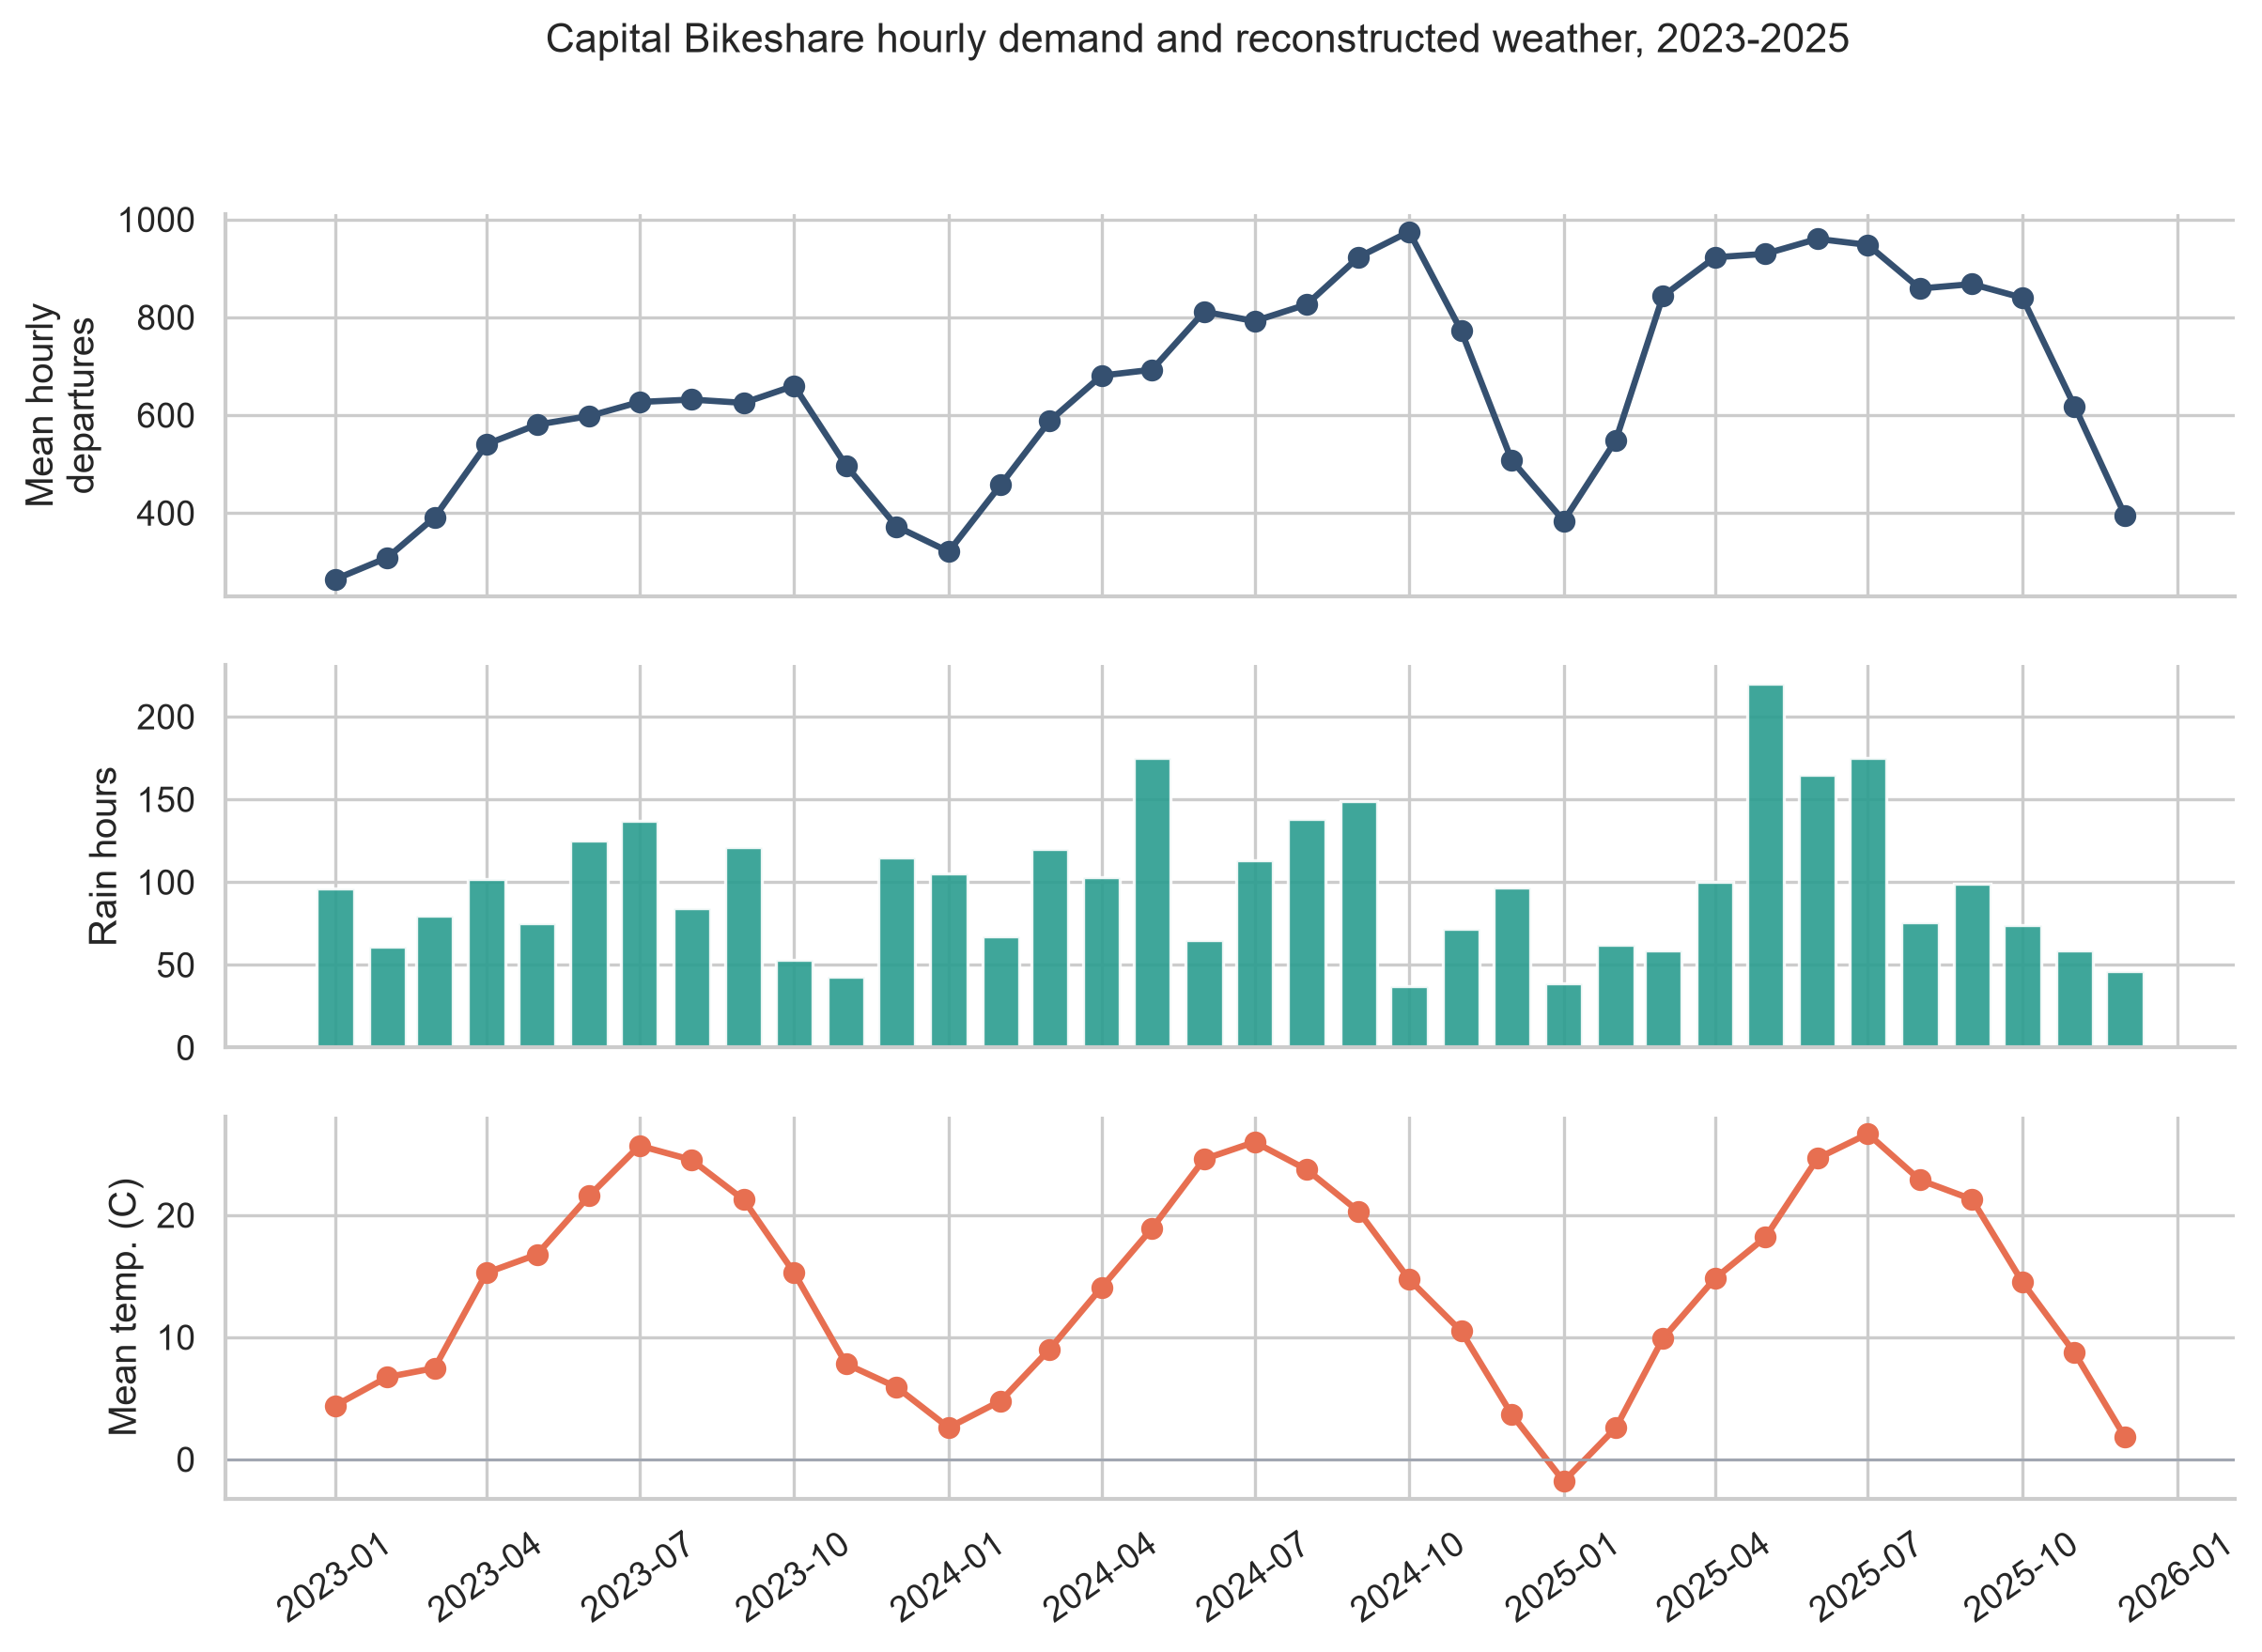
\includegraphics[width=0.98\textwidth]{assets/01_data_overview.png}
  \caption{2023--2025 年小时需求与历史天气重建的月度概况。需求季节性和温度季节性高度同步，因此图形只支持描述性关联，不支持因果结论。}
  \label{fig:data-overview}
\end{figure}

\subsection{预测任务与发布时间}

在小时 $t$ 的出发量聚合完成后发布预测，目标为
\begin{equation}
  Y_{t+h},\qquad h\in\{1,2,3,6\}.
\end{equation}
可用信息集合记为 $\mathcal{F}_t$。所有需求、天气和事件变量只能使用到 $t$；目标小时、星期、月份、节假日等日历变量可提前知道。任何包含 $Y_{t+h}$ 的训练行只有在最晚标签 $Y_{t+6}$ 到达后才能进入训练集。模型输出
\begin{equation}
  \widehat\mu_{t,h}=\mathbb{E}(Y_{t+h}\mid\mathcal{F}_t).
\end{equation}

\subsection{发布状态}

状态由发布时可见的在线雨事件解析器产生：
\begin{itemize}
  \item \textbf{正常状态（normal）：}发布时无进行中的降雨，且不在已确认事件后的恢复窗口；
  \item \textbf{冲击状态（shock）：}发布时降雨正在进行；
  \item \textbf{恢复状态（recovery）：}最近雨事件已经结束，且发布时仍处于预设恢复窗口。
\end{itemize}
状态只决定融合权重，不使用目标时刻的真实天气，也不利用未来事件结束时间或未来累计雨量。

\subsection{前向时间协议}

\begin{table}[H]
\centering
\caption{配置筛选、校准、融合与最终评价的连续前向切分}
\label{tab:splits}
\begin{tabularx}{0.92\textwidth}{lllX}
\toprule
阶段 & 发布时段 & 每时距样本 & 用途\\
\midrule
校准拟合（calibration fit） & 2024-01 至 2024-06 & 4,368 & 拟合每个专家的低维偏差校准\\
融合拟合（fusion fit） & 2024-07 至 2024-12 & 4,416 & 学习全局及三状态融合权重\\
筛选开发（screening dev） & 2025-01 至 2025-03 & 2,160 & 在 18 组候选中选择每类专家配置\\
最终评价（final evaluation） & 2025-04 至 2025-12 & 6,599 & 固定配置后的最终回溯评价\\
\bottomrule
\end{tabularx}
\end{table}

这种切分使最终评价不参与结构和超参数选择。补充确认实验复用已经冻结的六专家逐时预测，只重新拟合校准层、融合层和结构化 E3 变体；因此所有目标比较和 LOO 都保持同一专家预测输入，不通过最终评价期重新选择结构。

\section{动机验证：当前无雨时的降雨路径差异}
\label{sec:motivation}

\subsection{分组与检验方法}

为检验降雨历史是否对应需求基准尚未解释的残差差异，本文在模型冻结后进行补充诊断。分析使用最终评价区间的原始 E1 预测，选取当前雨量为零且满足下列条件之一的发布小时：
\begin{itemize}
  \item \textbf{连续干燥组：}过去 24 小时累计雨量为零，共 3,074 个小时；
  \item \textbf{近期降雨组：}过去第 3--12 小时累计雨量不少于 1 mm，最近 1--2 小时无雨，过去 24 小时累计雨量小于 5 mm，共 133 个小时；
  \item \textbf{强雨后初期组：}过去 12 小时累计雨量不少于 5 mm，且最近一次正降雨距发布时刻不超过 3 小时，共 248 个小时。
\end{itemize}
三组互不重叠，共包含 3,455 个发布小时、40 个日历周。这里的强雨后初期组对应动机实验文件中的 \texttt{recovery}，是按上述雨量与时间阈值选取的子组，区别于主模型的完整恢复状态。分组只读取发布时及以前的降雨。该诊断不参与专家配置、融合权重或主结果的选择。

定义有符号残差 $e_{t,h}=Y_{t+h}-\widehat\mu^{(1),\mathrm{raw}}_{t,h}$，正值表示 E1 低估出发量。分别以 $e_{t,h}$ 和 $|e_{t,h}|$ 为因变量，以连续干燥组为参照，拟合
\begin{equation}
 z_{t,h}=\beta_{0,h}+\beta_{1,h}I_{t,\mathrm{recent}}
 +\beta_{2,h}I_{t,\mathrm{postrain}}
 +a_{\mathrm{hour}(t+h)}+b_{\mathrm{weekday}(t+h)}
 +c_{\mathrm{month}(t+h)}+\varepsilon_{t,h}.
\end{equation}
其中 $z_{t,h}$ 分别取有符号残差与绝对残差，日历控制项按各时距的目标时间构造。采用日历周块 bootstrap 重采样 500 次，每次重新拟合控制回归，报告 95\% 百分位区间。

\subsection{残差差异与建模启示}

\begin{table}[H]
\centering
\caption{降雨路径相对连续干燥组的残差差异（控制目标小时、星期和月份）}
\label{tab:motivation}
\small
\begin{tabular}{llrr}
\toprule
对比组 & 时距/h & 有符号残差差异 [95\% CI] & 绝对残差差异 [95\% CI]\\
\midrule
近期降雨 & 1 & $-30.26\;[-66.57,8.68]$ & $-11.90\;[-32.83,16.12]$\\
近期降雨 & 2 & $-20.34\;[-50.25,16.88]$ & $-19.11\;[-35.78,5.24]$\\
近期降雨 & 3 & $-31.22\;[-73.95,7.77]$ & $-13.82\;[-36.16,19.01]$\\
近期降雨 & 6 & $-62.91\;[-92.38,-28.56]$ & $-23.43\;[-48.08,1.43]$\\
强雨后初期 & 1 & $-31.28\;[-62.55,0.68]$ & $-23.81\;[-39.31,-7.90]$\\
强雨后初期 & 2 & $-34.01\;[-62.38,2.24]$ & $-8.15\;[-29.85,10.86]$\\
强雨后初期 & 3 & $-35.09\;[-65.95,6.88]$ & $-9.84\;[-33.15,14.61]$\\
强雨后初期 & 6 & $-9.58\;[-51.58,42.93]$ & $7.41\;[-18.50,47.41]$\\
\bottomrule
\end{tabular}
\end{table}

近期降雨组的 6 小时有符号残差差异为 $-62.91$，95\% 区间为 $[-92.38,-28.56]$。原始平均残差也从连续干燥组的 72.75 降至近期降雨组的 7.57，表明 E1 在两组中的低估程度明显不同。强雨后初期组的 1 小时绝对残差差异为 $-23.81$，区间为 $[-39.31,-7.90]$，说明路径差异还体现在短时误差大小上。其余逐项区间均跨零，差异随预测时距和残差指标变化。

上述结果支持本文的核心判断：天气历史是值得单独组织的预测信息，当前无雨并不代表需求已回到同一种状态。路径差异既体现在残差方向，也体现在误差大小，因而适合由具有不同时间尺度的模型共同刻画。恢复专家显式表示降雨累积与雨后时间，时序专家从连续历史中学习变化模式，两类表示分别提供可解释的结构与灵活的时间依赖。这一分工将天气路径的经验发现转化为“专而治之”的建模方案。

\section{六专家完整预测框架}

\subsection{“专而治之”的总体设计}

六专家框架遵循“按信息分工、按能力建模、按状态融合”的设计原则。首先，将需求惯性、当前天气与历史恢复分别组织，避免每个专家都重复接收全部特征。其次，为局部变化、顺序累积和跨日依赖配置不同的轻量时序模型，使模型结构与所关注的时间模式对应。最后，在完整需求预测层面拟合组合权重，使各专家的优势能够共同用于同一预测任务。

这种分工落实在三个层面：输入上，需求、天气与恢复专家分别使用角色明确的变量；结构上，统计专家采用低自由度函数，深度专家采用浅层网络；融合上，每个时距和状态仅拟合六个组合权重。时序专家可以共享历史观测字段，但通过不同窗口和运算结构提取各自的表示。框架由此以受控的单专家规模组织复杂信息，将“汇集各模型优势”的目标落实为可训练、可比较的预测系统。


\subsection{共同输出尺度与负二项建模}

六个专家均预测完整的小时出发量，分别使用需求动态、当前天气、事件历史或时序表示。结构化专家显式指定变量与函数形式，深度专家从历史序列学习时间依赖。对于专家 $k$，
\begin{equation}
  Y_{t+h}\mid\mathcal{F}_t \sim \mathrm{NB}(\mu^{(k)}_{t,h},\alpha^{(k)}_h),
  \qquad \mathrm{Var}(Y_{t+h}\mid\mathcal{F}_t)=\mu^{(k)}_{t,h}+\alpha^{(k)}_h(\mu^{(k)}_{t,h})^2.
\end{equation}
每个深度专家内部由四个时距共享时序骨干网络，并设置对应的输出头。结构化专家按时距拟合，E1 则通过一个多输出树联合生成四维对数均值。

\begin{table}[H]
\centering
\caption{六个专家的独立建模贡献与最终选中配置}
\label{tab:experts}
\small
\begin{tabularx}{\textwidth}{c p{3.0cm} p{4.0cm} X}
\toprule
ID & 最终配置 & 专属贡献 & 主要输入和归纳偏置\\
\midrule
E1 & Multi-output NB-XGBoost & 需求自身动态与四时距联合基座 & 需求滞后、差分、滚动统计、目标日历；不直接输入天气\\
E2 & spline\_only & 当前天气的可解释非线性响应 & 发布时温度、降雨、湿度、风速的三次样条与公共控制\\
E3 & multi\_scale & 已结束雨事件的多尺度恢复记忆 & 事件累计雨量在 $\tau=3,12,36$ 小时尺度的衰减及在线事件字段\\
E4 & TCN, $L=72$, 32 通道, 3 块 & 局部因果、多尺度卷积模式 & 72 小时需求--天气序列，膨胀率 $1,2,4$\\
E5 & GRU, $L=72$, 隐藏维 64, 1 层 & 递归隐状态与顺序记忆 & 72 小时需求--天气序列，单层门控递归\\
E6 & Transformer, $L=168$, $d=32$, 1 层, 2 头 & 跨较远时刻的直接依赖 & 168 小时序列、可学习位置编码与轻量自注意力\\
\bottomrule
\end{tabularx}
\end{table}

\subsection{E1：需求自身动态贡献}

E1 采用多输出负二项 XGBoost。输入包含 $0,1,2,3,6,24,48,168$ 小时需求滞后、短期变化量、3/24/168 小时滚动均值和 24 小时滚动波动，以及四个目标时刻的日历特征。模型联合输出
\begin{equation}
  \bm\eta_t=(\eta_{t,1},\eta_{t,2},\eta_{t,3},\eta_{t,6}),\qquad
  \mu^{(1)}_{t,h}=\exp(\eta_{t,h}).
\end{equation}
E1 以需求自身变化和周期规律提供统一的预测基准。

\subsection{E2：TS-NBWE 当前天气非线性贡献}

E2 定义为张量样条负二项天气敏感专家（Tensor-Spline Negative-Binomial Weather Expert, TS-NBWE）。它刻画在发布时刻 $t$ 已经观测到的天气条件下，未来完整需求均值的非线性变化。E2 不读取历史天气序列、未来天气或尚未结束事件的未来总雨量，因而与 E1 的需求惯性、E3 的历史恢复记忆保持输入角色上的分离。

为防止天气变量在有限冲击样本上产生高自由度拟合，连续变量均采用低自由度三次 B 样条（cubic B-spline）。公共控制 $\bm c_{t,h}$ 只包含目标日历、发布小时与基本通勤标记，用来吸收可预知的时段差异。基础配置为
\begin{equation}
  \log\mu^{(2)}_{t,h}=\bm c_{t,h}^{\top}\bm\beta_h
  +s_T(T_t)+s_R\!\left(\log(1+R_t)\right)+s_H(H_t)+s_V(V_t),
  \label{eq:e2-base}
\end{equation}
其中 $T_t,R_t,H_t,V_t$ 分别表示发布时温度、雨量、湿度与风速。负二项对数似然使模型直接适配计数需求的过度离散，而样条基函数允许冷、热、小雨和强雨附近具有不同局部斜率，用于描述给定日历条件下的天气与需求关系。

E2 的候选设计逐层增加交互复杂度。\texttt{spline\_only} 只含式~\eqref{eq:e2-base}；\texttt{spline\_th} 增加温度--湿度张量项 $s_{TH}(T_t,H_t)$；\texttt{full\_tensor} 再加入雨量--风速张量项 $s_{RV}(R_t,V_t)$ 与通勤时段雨量响应。三种方案的开发期相对选择分数分别为 0.877039、0.877200 和 0.879186，数值越小越好。\texttt{spline\_only} 的开发期分数最低，且增加交互项未带来改善，因此选择一维样条配置。

E2 在模型结构上提供当前天气的低维平滑表示，在增量实验中主要改善 1 小时预测，并在短时冲击状态保留一定融合权重。其预测价值集中于短时天气校正。

\subsection{E3：MSER-NB 多尺度事件恢复贡献}

E3 定义为多尺度事件恢复负二项专家（Multi-Scale Event-Recovery Negative-Binomial Expert, MSER-NB），刻画已发生的降雨过程与后续需求的关系。在线事件解析器在每个发布时刻更新降雨状态、已持续时长、当前累计雨量，以及最近一个已结束事件的摘要，所有字段均由当时已知的观测构造。

对最近已结束事件，记累计雨量、持续时长和雨停后经过时间为 $C_t,D_t,S_t$。为避免预先假定唯一恢复速度，E3 构造三个衰减尺度：
\begin{align}
  E^{C,\tau}_{t,h}&=\log(1+C_t)\exp\!\left[-\frac{\min(S_t+h,72)}{\tau}\right],\\
  E^{D,\tau}_{t,h}&=\log(1+D_t)\exp\!\left[-\frac{\min(S_t+h,72)}{\tau}\right],
  \qquad \tau\in\{3,12,36\}.
  \label{eq:e3-decay}
\end{align}
$\tau=3$ 描述快速回弹，$\tau=12$ 描述日内恢复，$\tau=36$ 则允许影响跨越一个自然日。该设计把“雨后恢复”从固定 12 小时窗口改为可由数据组合的多时间尺度表示，同时保证式中每一项都能在发布时计算。

除事件摘要外，候选设计还测试连续雨历史记忆：
\begin{equation}
  M^{\tau}_{t,h}=\sum_{\ell=1}^{72}\log(1+R_{t-\ell})
  \exp\!\left[-\frac{\ell+h}{\tau}\right],
  \qquad \tau\in\{3,12,36\}.
  \label{eq:e3-memory}
\end{equation}
这里的 $M^{\tau}_{t,h}$ 不需要把历史小时硬切成单一雨事件，可表达多段小雨或间歇降雨的累积记忆。候选 \texttt{multi\_scale} 使用式~\eqref{eq:e3-decay} 的已结束事件摘要；\texttt{memory} 加入式~\eqref{eq:e3-memory}；\texttt{full} 再加入事件持续时长及累计雨量--时长交互。初始开发期相对选择分数依次为 0.887374、0.887571 和 0.887576，最终按开发期规则选择结构更简单的 \texttt{multi\_scale}。

补充确认中另构造 \texttt{history\_only}：移除当前天气与进行中降雨字段，只保留公共控制、已结束事件摘要和连续历史记忆。四种 E3 设计在最终期的四时距平均 MAE 为 104.875--104.888，恢复状态为 106.741--106.767，差异很小。因此正文继续采用事先冻结的 \texttt{multi\_scale}，不根据最终期的微小差异改选配置。E3 提供已发生降雨事件的多尺度表示；其在融合中的边际价值由后文消融结果检验。

\subsection{E4：TCN 局部多尺度贡献}

E4 读取过去 72 小时的需求、温度、降雨、湿度、风速、冲击/恢复指示、事件持续字段和周期编码。三层因果卷积块的膨胀率为 $1,2,4$，每块采用残差连接：
\begin{equation}
  \bm z^{(l)}=\bm z^{(l-1)}+\mathrm{Dropout}\{\mathrm{ReLU}(\mathrm{Conv}_{d_l}(\bm z^{(l-1)}))\}.
\end{equation}
E4 的贡献是学习人工滞后和事件衰减没有直接指定的局部、多尺度时序形状。最终配置包含 9,956 个参数。

\subsection{E5：GRU 顺序状态贡献}

E5 使用与 E4 相同的 72 小时序列字段，但将历史压缩为门控递归状态：
\begin{equation}
  \bm h_t=\mathrm{GRU}(\bm x_{t-71:t}),\qquad
  \bm\eta_t=\bm W\bm h_t+\bm b.
\end{equation}
其独立贡献是检验显式递归状态是否适合表示需求和天气过程的顺序累积。最终配置为单层、隐藏维度 64，共 15,812 个参数。

\subsection{E6：Tiny Transformer 长距离依赖贡献}

E6 采用 168 小时窗口，每小时构成一个需求--天气--事件词元（token）。线性投影和可学习位置编码后，通过一层双头 Transformer 编码器（encoder）：
\begin{equation}
  \bm Z=\mathrm{Encoder}(\bm X\bm W_e+\bm P),\qquad
  \bm\eta_t=\bm W_o\bm Z_{t}+\bm b_o.
\end{equation}
E6 的贡献是允许一周窗口内相隔较远的时间点直接交互，而不依赖卷积层数或递归传递。最终配置 $d_{\text{model}}=32$、FFN=64、1 层、2 头，共 14,564 个参数。

\subsection{专家校准与权重联合优化}

轻量融合是“专而治之”连接独立建模与整体预测的关键。基础六专家实现采用 Softmax 将六个可学习分数映射为归一化权重：
\begin{equation}
 w_{h,s,k}=\frac{\exp(z_{h,s,k})}{\sum_{j=1}^{6}\exp(z_{h,s,j})},
 \qquad k=1,\ldots,6.
 \label{eq:softmax-fusion}
\end{equation}
训练时以组合预测误差为目标，通过 L-BFGS-B 迭代更新分数。每个时距和状态只需优化六个分数，融合层保持低维结构，同时自动满足权重为正、和为一的条件。这使专家能够独立设计和训练，再以很小的融合参数规模共同参与预测。后续确认实验使用 SLSQP 直接求解非负归一化权重，以统一比较融合损失与消融配置；两种实现均遵循低维加权组合的设计。

每个专家先在 calibration fit 上进行低维偏差校准：
\begin{equation}
  \widetilde\mu^{(k)}_{t,h}=\max\{0,a_{k,h}+b_{k,h}\mu^{(k)}_{t,h}\}.
\end{equation}
在 fusion fit 上学习全局权重，再对每个状态学习向全局权重收缩的状态权重：
\begin{align}
  \widehat\mu^{(F)}_{t,h}&=\sum_{k=1}^{6}w_{h,s_t,k}\widetilde\mu^{(k)}_{t,h},\\
  \min_{\bm w}\quad &\frac{1}{n_s q_{h,s}^2}\sum_{t:s_t=s}\left(Y_{t+h}-\sum_{k=1}^{6}w_k\widetilde\mu^{(k)}_{t,h}\right)^2
  +\lambda\lVert\bm w-\bm w_h^{(G)}\rVert_2^2,\\
  \text{s.t.}\quad &w_k\ge 0,\qquad \sum_{k=1}^{6}w_k=1.
\end{align}
其中 $q_{h,s}$ 为拟合样本中目标绝对值均值与 1 的较大值，用于统一损失尺度；状态收缩系数取 $\lambda=0.5$。实现采用基于梯度信息的序列最小二乘规划（SLSQP），在非负且和为一的约束下迭代优化权重。先拟合全局组合，再以全局权重为中心拟合状态组合，使小样本状态也能借助整体信息保持稳定。

权重针对六个专家的联合预测误差拟合，因此不仅反映单个专家的精度，也利用专家之间的误差互补。不同状态下贡献较小的专家可以获得较低或零权重，同时仍保留在专家集合中。这样，六类建模能力由框架统一提供，具体预测中各类能力的使用程度由数据决定。

\subsection{滚动经验预测区间}

对完整融合预测定义异方差归一化残差
\begin{equation}
  r_{t,h}=\frac{|Y_{t+h}-\widehat\mu^{(F)}_{t,h}|}{\max\{\sqrt{\widehat\mu^{(F)}_{t,h}},25\}}.
\end{equation}
在发布时刻 $t$，只纳入目标时间不晚于 $t$ 的既往残差，并保留最近 2,160 个分数。令 $q_{t,h,\gamma}$ 为经验 $\gamma$ 分位数，则
\begin{equation}
  \left[\max\{0,\widehat\mu^{(F)}_{t,h}-q_{t,h,\gamma}s_{t,h}\},
  \widehat\mu^{(F)}_{t,h}+q_{t,h,\gamma}s_{t,h}\right],
  \quad s_{t,h}=\max\{\sqrt{\widehat\mu^{(F)}_{t,h}},25\}.
\end{equation}
滚动更新使区间能够随近期预测误差调整，适应需求波动和天气状态的变化。

\section{实验设置}

\subsection{候选筛选与完整模型训练}

E1 作为固定需求基准，不参与结构搜索。E2 和 E3 各测试 3 种配置，E4、E5、E6 各测试 4 种配置，共 18 组。各类专家先根据 2025 年第一季度开发期表现确定配置，再与 E1 分别组合，评估相对需求基准的独立增量。随后使用选定配置训练六类专家，拟合完整融合模型。

在冻结上述配置后，补充确认实验执行四项检查。第一，分别移除 E2--E6，并对剩余专家重新拟合校准与融合，得到去一专家消融（leave-one-expert-out, LOO）；E1 作为问题基座始终保留。第二，只用 screening dev 比较 MSE、MAE、Huber 和状态加权 Huber 的融合敏感性，final evaluation 不参与选择。第三，分别以统一残差池和 normal/shock/recovery 状态残差池构造滚动分位数。第四，重拟合 E3 的四种结构变体，检查结论是否依赖单一事件表示。深度专家预测保持冻结，不在确认实验中改变网络或随机种子。

实验在 CPU 环境下运行，使用 PyTorch 2.14.0。三个深度专家分别采用 3 个卷积块、1 层 GRU 和 1 层 Transformer，参数量为 9,956、15,812 和 14,564，合计 40,332。表~\ref{tab:engineering}列出各模型实际耗时。结合低自由度统计专家与六维融合权重，这一配置将“专而治之”落实为可在 CPU 环境运行的轻量系统。

\begin{table}[H]
\centering
\caption{轻量时序专家的参数规模与运行耗时}
\label{tab:engineering}
\begin{tabular}{lrrr}
\toprule
专家 & 参数量 & 训练时间/s & 推理时间/s\\
\midrule
E4 TCN & 9,956 & 219.987 & 0.225\\
E5 GRU & 15,812 & 392.004 & 0.935\\
E6 Tiny Transformer & 14,564 & 1,661.360 & 1.015\\
\bottomrule
\end{tabular}
\end{table}


\subsection{评价指标}

点预测使用
\begin{align}
  \mathrm{MAE}&=\frac{1}{n}\sum_{i=1}^{n}|y_i-\widehat y_i|,\\
  \mathrm{RMSE}&=\sqrt{\frac{1}{n}\sum_{i=1}^{n}(y_i-\widehat y_i)^2}.
\end{align}
同时按正常（normal）、冲击（shock）、恢复（recovery）分组。区间报告经验覆盖率和平均宽度。LOO 定义
\begin{equation}
  \Delta\mathrm{MAE}_{-k}=\mathrm{MAE}(\mathcal E\setminus\{k\})-\mathrm{MAE}(\mathcal E),
\end{equation}
正值表示专家 $k$ 在其余专家均存在时仍能降低误差。正常与总体样本使用日历周块 bootstrap，shock/recovery 使用事件簇 bootstrap，均重复 500 次并报告 95\% 区间。该口径不同于 E1 加单专家：前者衡量完整模型中的边际增益，后者衡量相对固定基准的独立增量。

\section{单专家增量贡献}

\begin{table}[H]
\centering
\caption{每个候选专家单独加入 E1 后的最终期增量价值}
\label{tab:incremental}
\small
\begin{tabular}{lrrrrrr}
\toprule
模型 & 1h MAE & 2h MAE & 3h MAE & 6h MAE & 平均 MAE & 相对 E1 改善\\
\midrule
E1 only & 130.964 & 143.024 & 165.942 & 173.002 & 153.233 & --\\
E1+E2 Weather & 105.030 & 144.064 & 168.051 & 182.537 & 149.921 & 2.16\%\\
E1+E3 Recovery & 104.626 & 143.407 & 166.750 & 179.929 & 148.678 & 2.97\%\\
E1+E4 TCN & 78.756 & 99.890 & 118.169 & 129.846 & 106.665 & 30.39\%\\
E1+E5 GRU & 80.401 & 104.157 & 122.759 & 140.543 & 111.965 & 26.93\%\\
E1+E6 Transformer & 106.175 & 121.432 & 138.529 & 148.851 & 128.747 & 15.98\%\\
\bottomrule
\end{tabular}
\end{table}

\begin{figure}[H]
  \centering
  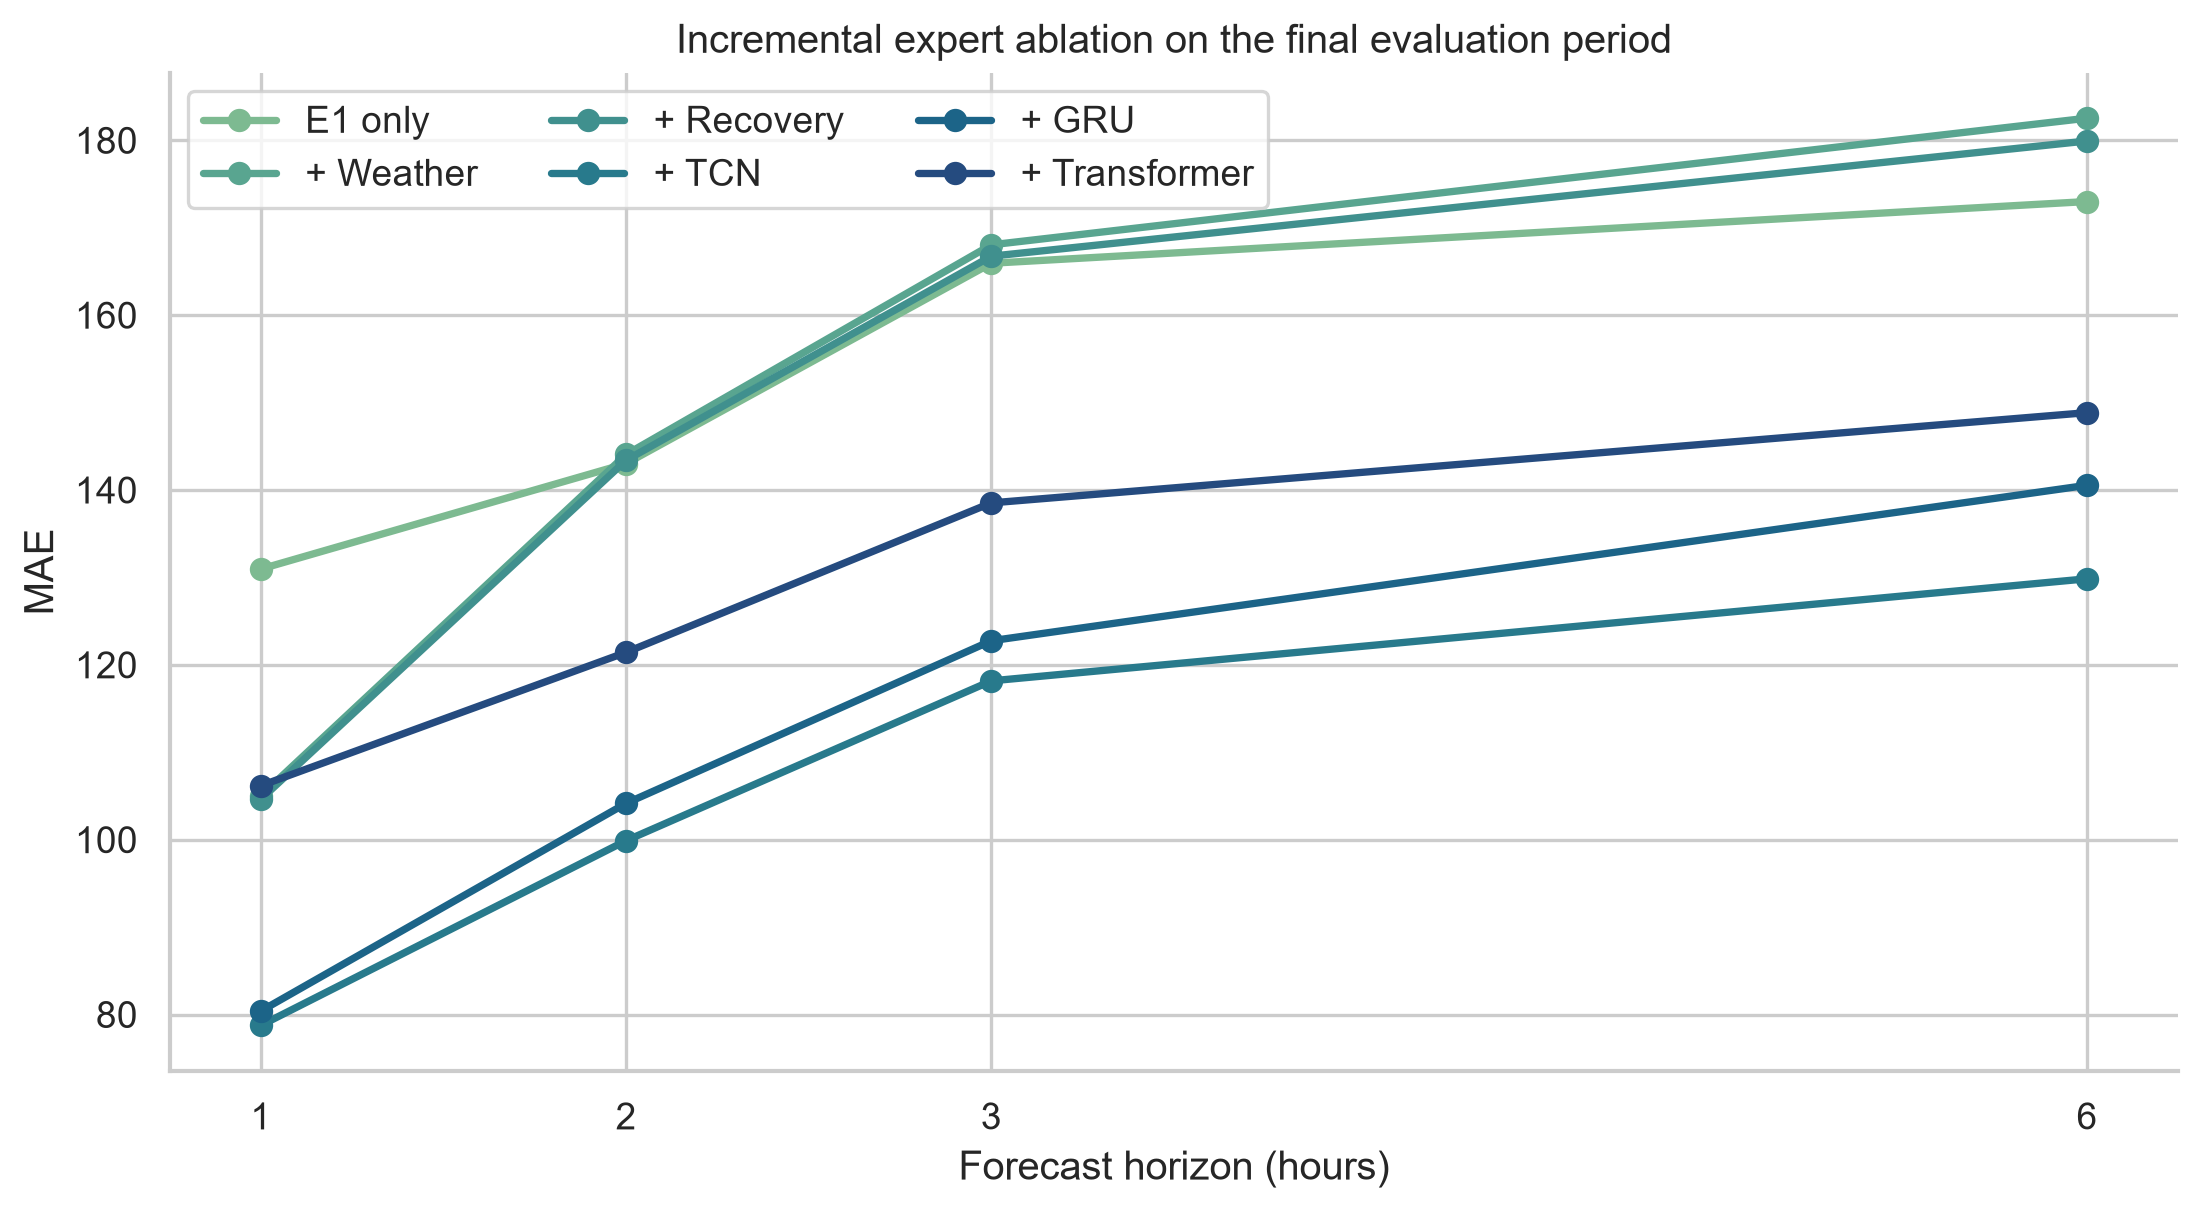
\includegraphics[width=0.98\textwidth]{assets/02_incremental_ablation.png}
  \caption{固定 E1 后分别加入一个候选专家的四时距 MAE。E4 和 E5 带来最大整体改善；E2 与 E3 的主要增益集中在 1 小时。}
  \label{fig:incremental}
\end{figure}

表~\ref{tab:incremental}显示，E2 和 E3 分别将 1 小时 MAE 降低 19.80\% 和 20.11\%，但在 2--6 小时未改善基准，增益集中于短时预测。E4 在全部时距大幅降低误差，是单专家增量最大的方案；E5 次之；E6 也在四个时距一致改善 E1。这些比较直接衡量各专家与同一需求基准组合后的预测价值。

\section{六专家完整模型结果}

\subsection{总体点预测}

\begin{table}[H]
\centering
\caption{六专家完整模型在最终评价区间的总体点预测结果}
\label{tab:full-overall}
\begin{tabular}{rrrrr}
\toprule
时距/h & 样本数 & MAE & RMSE & 目标均值\\
\midrule
1 & 6,599 & 75.691 & 117.124 & 815.271\\
2 & 6,599 & 97.794 & 156.000 & 815.286\\
3 & 6,599 & 116.644 & 187.735 & 815.291\\
6 & 6,599 & 129.372 & 203.462 & 815.376\\
\bottomrule
\end{tabular}
\end{table}

六专家融合的四时距平均 MAE 为 104.875，相对 E1 的 153.233 降低 31.56\%。相比表现最好的单专家增量方案 E1+TCN（106.665），完整融合进一步降低平均 MAE 约 1.68\%，且在四个时距均取得更低误差。这表明多个预测视角的组合能在强增量方案基础上继续改善预测。各专家在完整模型中的边际作用见第~\ref{sec:loo}节。

\subsection{融合目标敏感性}

原设计以 MSE 学习融合权重，而正文主要报告 MAE。为检查两种口径是否冲突，确认实验在不改变专家预测的前提下比较四种融合目标。MAE 目标在 screening dev 的综合选择分数为 0.997065，相对 MSE 的 1.000000 仅改善 0.294\%；状态加权 Huber 为 0.998391，普通 Huber 为 1.000319。主结果沿用预设 MSE，其余目标用于敏感性分析。

\begin{table}[H]
\centering
\caption{四种融合目标在最终评价期的四时距平均误差}
\label{tab:fusion-objectives}
\begin{tabular}{lrr}
\toprule
融合目标 & 平均 MAE & 平均 RMSE\\
\midrule
MSE（主结果） & \textbf{104.875} & \textbf{166.080}\\
MAE & 105.167 & 166.670\\
Huber & 105.131 & 166.611\\
状态加权 Huber & 105.274 & 166.604\\
\bottomrule
\end{tabular}
\end{table}

\begin{figure}[H]
  \centering
  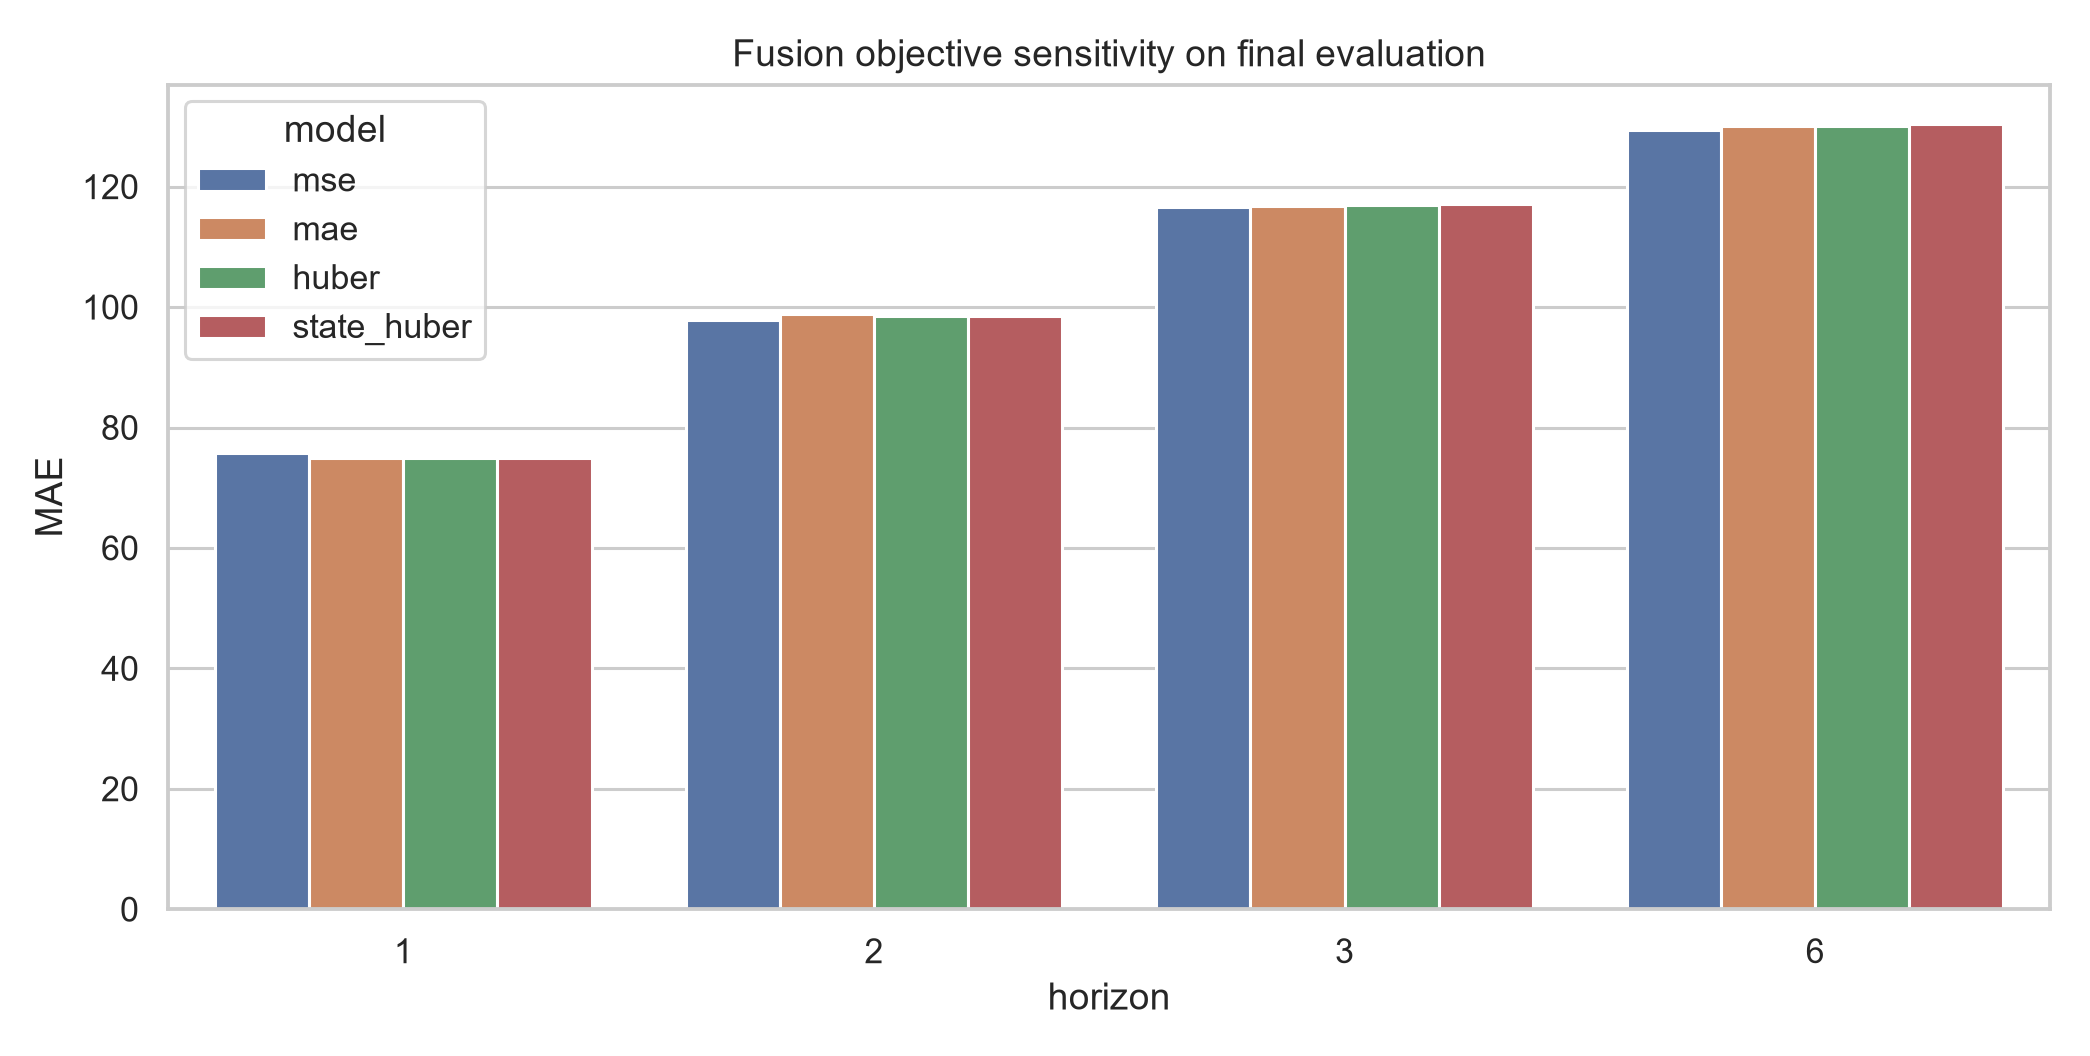
\includegraphics[width=0.96\textwidth]{assets/11_fusion_objectives.png}
  \caption{冻结六专家预测后的融合目标敏感性。图中 final evaluation 只用于报告，不用于选择目标。}
  \label{fig:fusion-objectives}
\end{figure}

\subsection{状态分组误差}

\begin{table}[H]
\centering
\caption{六专家完整模型按发布状态分组的 MAE}
\label{tab:state-mae}
\begin{tabular}{lrrrrr}
\toprule
发布状态 & 样本数/时距 & 1h & 2h & 3h & 6h\\
\midrule
正常（normal） & 3,074 & 66.527 & 84.260 & 101.204 & 111.791\\
冲击（shock） & 1,018 & 102.785 & 137.129 & 158.274 & 171.169\\
恢复（recovery） & 2,507 & 75.925 & 98.417 & 118.672 & 133.956\\
\bottomrule
\end{tabular}
\end{table}

冲击状态在所有时距下最难，四时距平均 MAE 为 142.339；恢复状态为 106.743，正常状态为 90.945。冲击状态对应更高的点预测误差，区间校准需要适应该状态的误差尺度。

\subsection{六专家预测份额}

\begin{table}[H]
\centering
\caption{MSE 完整模型的全局预测权重}
\label{tab:global-weights}
\begin{tabular}{rrrrrrr}
\toprule
$h$ & E1 & E2 & E3 & E4 & E5 & E6\\
\midrule
1 & 0.036 & 0.094 & 0.000 & 0.271 & 0.469 & 0.130\\
2 & 0.000 & 0.000 & 0.000 & 0.406 & 0.254 & 0.341\\
3 & 0.000 & 0.007 & 0.000 & 0.331 & 0.251 & 0.411\\
6 & 0.000 & 0.000 & 0.010 & 0.307 & 0.275 & 0.408\\
\bottomrule
\end{tabular}
\end{table}

全局权重显示：1 小时主要由 E5、E4 和 E6 构成，同时 E2 保留 0.094；2 小时主要由 E4、E6 和 E5 构成；3 小时和 6 小时的最大全局份额均为 E6。状态权重受到 $\lambda=0.5$ 的全局收缩，各状态的典型权重为：1h shock 的 E2 为 0.100，3h shock 的 E3 为 0.012，6h shock 的 E3/E6 分别为 0.028/0.415。由此，权重只说明融合器在给定状态下如何组合预测，专家的边际增益则由 LOO 进一步检验。

\subsection{去一专家消融：完整模型中的边际作用}
\label{sec:loo}

E1 加单专家实验衡量各视角相对需求基准的增量，去一专家消融进一步衡量其在完整模型中的作用。表~\ref{tab:loo}报告逐一移除 E2--E6、重新拟合校准与融合后的误差变化。

\begin{table}[H]
\centering
\caption{去一专家后总体 MAE 的变化（LOO $-$ full；正值表示被移除专家有帮助）}
\label{tab:loo}
\small
\begin{tabular}{lrrrrr}
\toprule
移除专家 & 1h & 2h & 3h & 6h & 四时距平均\\
\midrule
E2 TS-NBWE & -0.066 & -0.006 & -0.079 & -0.010 & -0.040\\
E3 MSER-NB &  0.002 & -0.009 &  0.015 & -0.030 & -0.006\\
E4 TCN & 5.157 & 9.591 & 7.119 & 8.208 & 7.519\\
E5 GRU & 5.429 & 2.886 & 2.982 & 2.236 & 3.383\\
E6 Transformer & -0.957 & -1.444 & -0.882 & 1.475 & -0.452\\
\bottomrule
\end{tabular}
\end{table}

\begin{figure}[H]
  \centering
  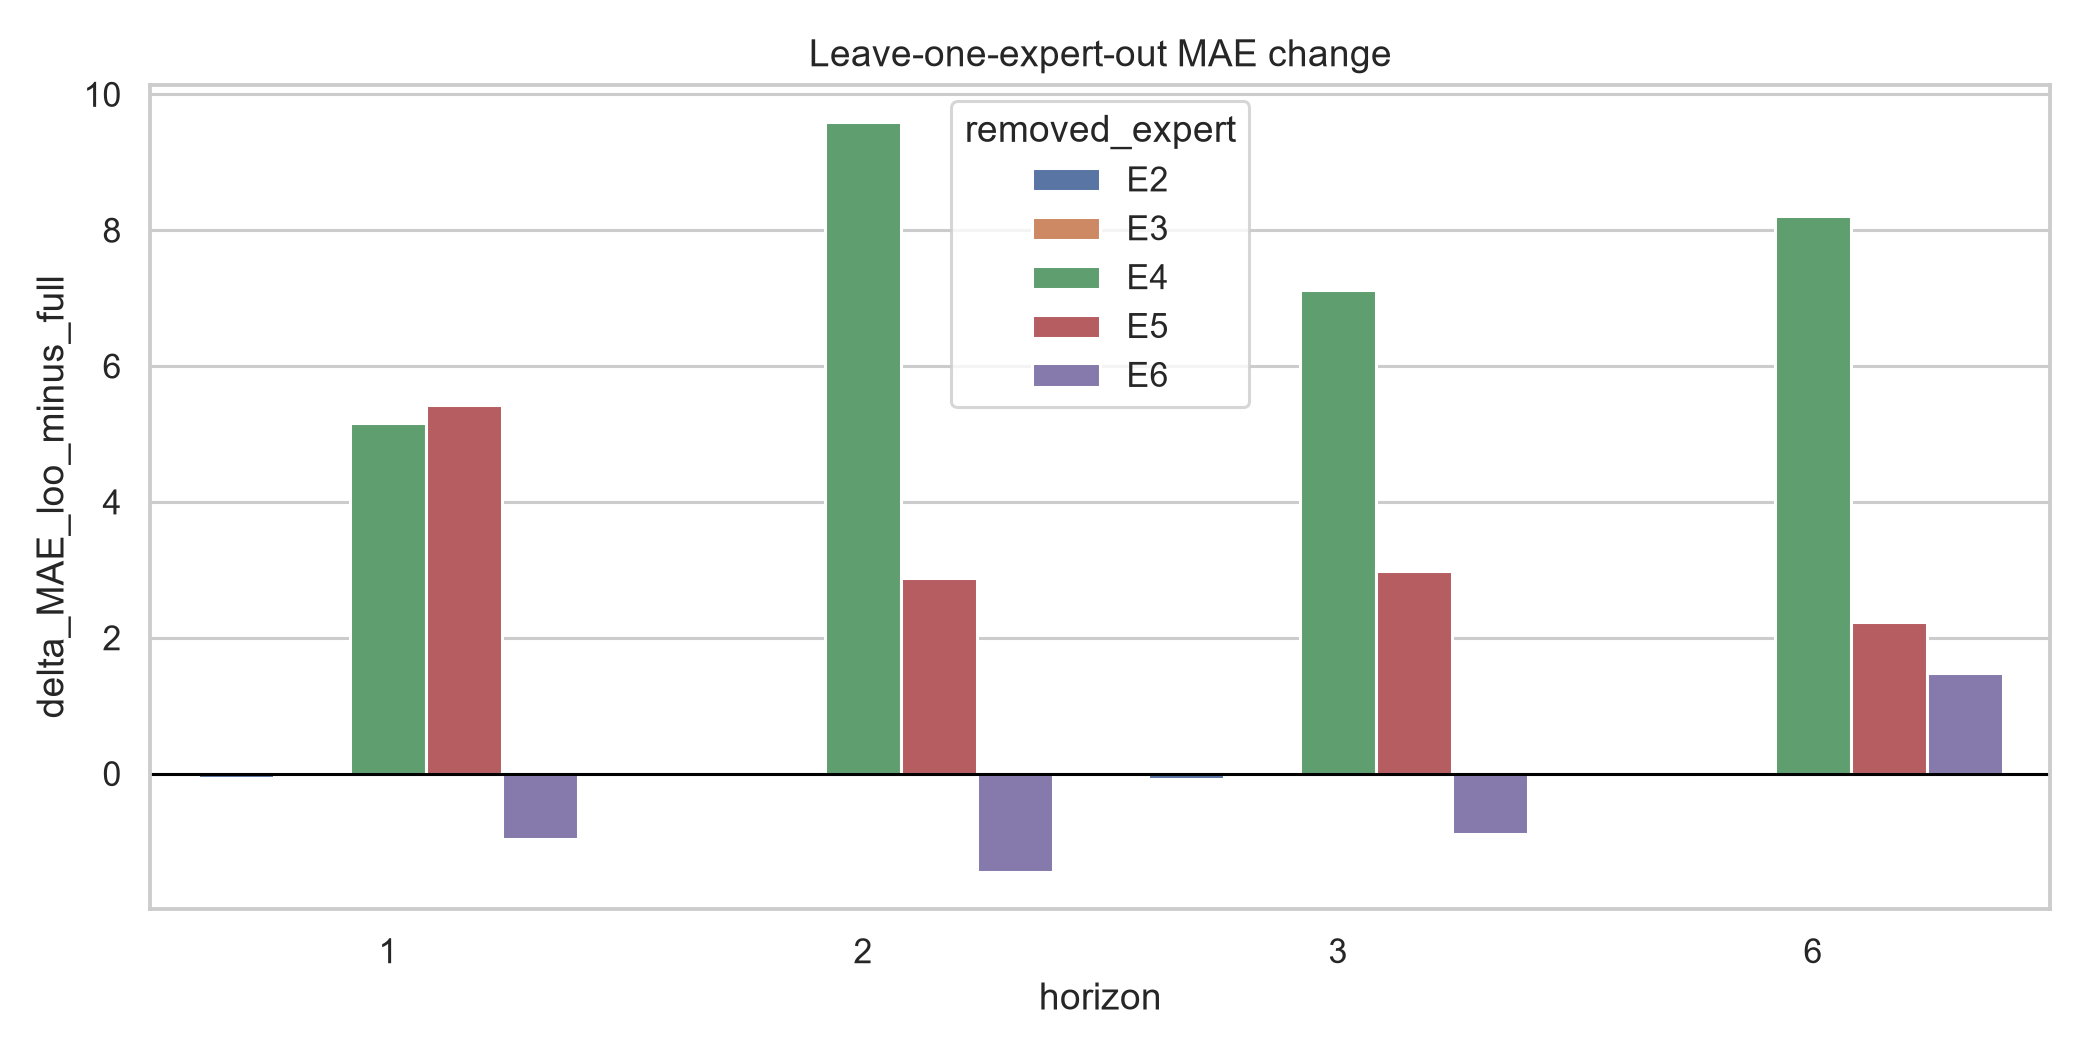
\includegraphics[width=0.98\textwidth]{assets/12_leave_one_out.png}
  \caption{去一专家消融的逐时距总体 MAE 变化。E4 和 E5 在全部时距均保持正边际作用；E6 的作用随时距变化。}
  \label{fig:loo}
\end{figure}

E4 的四个时距 95\% 周块 bootstrap 区间分别为 $[4.368,5.929]$、$[7.977,11.347]$、$[5.369,8.616]$ 和 $[6.281,10.157]$；E5 分别为 $[4.278,6.327]$、$[2.293,3.569]$、$[2.104,3.877]$ 和 $[0.508,3.844]$，均高于零。TCN 与 GRU 因而构成完整模型中跨时距稳定的增益来源。E2、E3 的总体变化接近零，在冲击状态的平均变化分别为 0.096 和 0.016。E6 的边际作用具有时距差异：移除后 1--3 小时总体误差略降，6 小时误差上升 1.475。其移除后的四时距平均 MAE 约为 104.423，略低于完整模型的 104.875；完整模型则保留了 E6 对 6 小时预测的改善。

\section{滚动经验预测区间}

统一滚动分位数的总体覆盖接近名义水平，但它把 normal 的低波动与 shock 的高波动放在同一个残差池中，导致正常状态偏宽、冲击状态偏窄。补充实验保持完全相同的 issue-time 更新规则，只把历史残差按发布状态分别入池；当某状态早期样本不足时回退到全局池，避免使用未来分数。

\begin{table}[H]
\centering
\caption{全局与状态分位数区间的四时距平均表现}
\label{tab:interval}
\small
\begin{tabular}{llrrrr}
\toprule
方法 & 状态 & 90\% 覆盖 & 90\% 宽度 & 95\% 覆盖 & 95\% 宽度\\
\midrule
全局（global） & overall & 0.900 & 436.943 & 0.949 & 580.694\\
全局（global） & normal & 0.927 & 425.948 & 0.968 & 563.630\\
全局（global） & shock & 0.818 & 448.754 & 0.884 & 597.433\\
全局（global） & recovery & 0.900 & 445.628 & 0.951 & 594.819\\
\midrule
状态分位数 & overall & 0.907 & 454.287 & 0.955 & 595.722\\
状态分位数 & normal & 0.905 & 383.663 & 0.956 & 497.483\\
状态分位数 & shock & 0.914 & 683.510 & 0.956 & 892.663\\
状态分位数 & recovery & 0.907 & 447.803 & 0.954 & 595.604\\
\bottomrule
\end{tabular}
\end{table}

\begin{figure}[H]
  \centering
  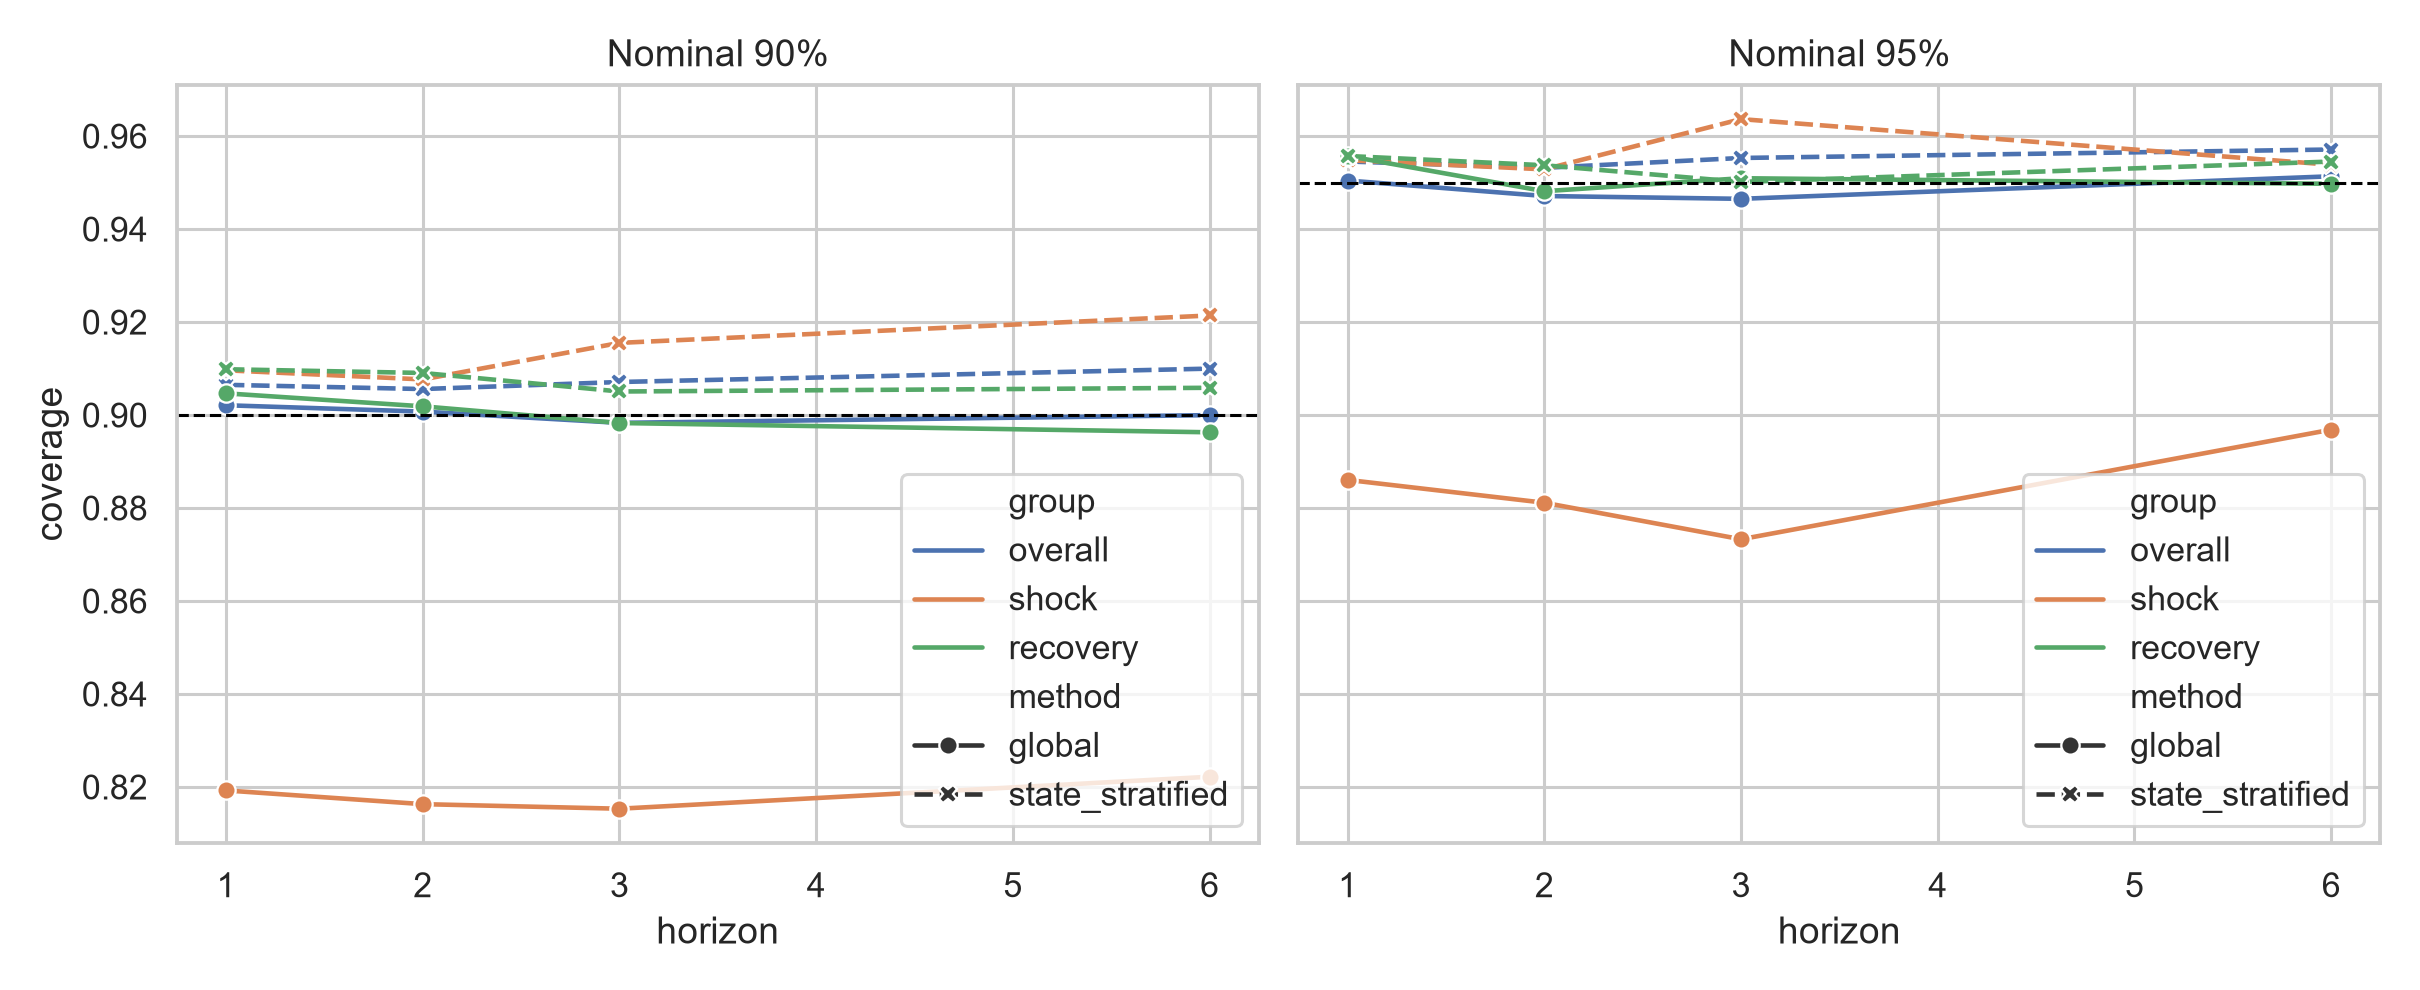
\includegraphics[width=0.99\textwidth]{assets/13_state_intervals.png}
  \caption{全局残差池（实线圆点）与状态残差池（虚线叉号）的滚动覆盖率。黑色虚线表示名义覆盖。}
  \label{fig:interval-coverage}
\end{figure}

状态分位数将冲击状态的平均 90\%/95\% 覆盖率分别从 0.818/0.884 提高到 0.914/0.956，事件簇 bootstrap 的逐时距结果也支持这一改善；对应的平均宽度增加 52.3\%/49.4\%。在正常状态下，90\% 区间平均宽度从 425.948 缩小到 383.663，覆盖率从 0.927 调整到更接近名义水平的 0.905。分状态校准由此改善了冲击期覆盖和正常期区间锐度，使区间宽度更符合不同状态的误差水平。

\section{讨论}

\subsection{专家分工与预测贡献}

E1 提供需求惯性与日周周期参照。E2 刻画发布时天气的非线性关系，E3 表示已结束降雨事件的多尺度历史，两者与 E1 组合时均改善 1 小时预测。TCN 和 GRU 分别通过局部卷积与递归状态形成稳定互补，在完整模型的全部时距均有正边际贡献。Transformer 在较长时距发挥作用，6 小时预测对其依赖更为明显。

增量实验与消融实验从两个层面验证架构：单专家增量比较表明，每类专家都能在至少一个时距补充需求基准；完整模型消融进一步揭示，不同专家承担的作用随时距和状态变化。TCN 与 GRU 构成稳定的预测主力，天气、恢复与注意力专家保留更具针对性的建模能力。这样的分工使框架能够同时利用稳定规律与条件性信息。

\subsection{降雨历史与时序表示的互补性}

动机实验首先确认：在当前无雨的样本中，历史降雨路径仍与需求基准的残差有关。结构化天气与恢复专家随后在 1 小时增量比较中降低误差，说明专门组织天气信息能够补充需求基准。完整模型的消融结果进一步表明，TCN 与 GRU 已吸收相当一部分相关时序信息，使 E2、E3 的额外边际作用缩小。这些结果形成了从残差差异、单专家增量到融合边际作用的证据链，支持联合考察显式天气历史和学习型时间表示。

\subsection{保留六专家的完整性与适用性}

六专家的分工同时体现在信息与模型两个层面：前三类专家分别组织需求、当前天气和恢复历史，后三类专家通过卷积、递归与注意力学习不同时间依赖。轻量融合将这六种能力接入统一输出，使框架既保留各专家的独立角色，又能根据实际误差调整其使用程度。围绕该架构，动机验证、候选筛选、增量比较、去一专家消融、融合目标敏感性、恢复结构变体和状态区间实验分别检验不同环节，构成本文较为完整的实证验证体系。

本文保留六类专家，是为了完整覆盖需求规律、当前天气、恢复历史和不同时间尺度的表示能力。某类专家在当前样本中的使用程度较低，并不改变它在整体设计中承担的信息角色。将完整专家集合与自适应权重结合，能够使模型根据天气状态和预测时距选择组合，同时为不同数据条件下的应用保留相应建模入口。这里的完整性指六类信息与模型能力的覆盖，通用性则体现为同一套分工与融合流程可用于组织不同场景的数据。

完整融合的平均 MAE 比 E1 基准降低 31.56\%，比最强单专家增量方案 E1+TCN 进一步降低 1.68\%，且四个时距均得到改善。结合三个深度专家合计约 4 万个参数的配置，结果表明，小型异构专家可以通过联合权重拟合形成有效组合。本文所追求的“集各家之长”由此体现为明确的信息分工、受控的模型规模和实际的预测提升。

\section{结论}

本文从“当前天气相近，历史天气路径不同，需求表现仍有差异”这一现象出发，将天气路径与雨后恢复纳入共享单车需求建模。当前无雨条件下的动机实验发现，近期降雨组在 6 小时时距的有符号残差比连续干燥组低 62.91，95\% 周块 bootstrap 区间不含零，支持单独组织天气历史信息。在此基础上，本文提出“专而治之”的六专家架构，将需求动态、当前天气、恢复记忆与三类时序表示分别交由不同模型处理，并通过状态权重联合优化实现优势互补。

在 Capital Bikeshare 2025 年 4--12 月的最终评价中，六专家融合在 1、2、3、6 小时的 MAE 分别为 75.691、97.794、116.644 和 129.372，平均 MAE 为 104.875，比 E1 基准降低 31.56\%，比最强单专家增量方案 E1+TCN 进一步降低 1.68\%。增量与消融实验验证了不同建模视角的互补价值，其中 TCN 与 GRU 提供跨时距稳定增益，其余专家形成面向特定信息和时间尺度的补充。三个深度专家合计仅 40,332 个参数，完整实验在 CPU 环境运行，体现了轻量建模与组合精度的兼顾。状态分位数校准进一步改善冲击期覆盖与正常期区间锐度。由天气路径发现出发，以专门化分工控制模型规模，再以联合优化汇集各专家优势，这一建模思路在本研究的多时距需求预测中取得了有效的实证支持。

\appendix
\section{完整模型状态权重明细}

\begin{longtable}{rlrrrrrr}
\caption{六专家在各时距和发布状态下的预测权重}\label{tab:weights-full}\\
\toprule
$h$ & 状态 & E1 & E2 & E3 & E4 & E5 & E6\\
\midrule
\endfirsthead
\toprule
$h$ & 状态 & E1 & E2 & E3 & E4 & E5 & E6\\
\midrule
\endhead
1 & normal & 0.036 & 0.092 & 0.000 & 0.272 & 0.471 & 0.129\\
1 & shock & 0.040 & 0.100 & 0.006 & 0.265 & 0.463 & 0.127\\
1 & recovery & 0.035 & 0.095 & 0.001 & 0.271 & 0.467 & 0.130\\
2 & normal & 0.000 & 0.000 & 0.000 & 0.407 & 0.254 & 0.340\\
2 & shock & 0.011 & 0.007 & 0.004 & 0.392 & 0.253 & 0.332\\
2 & recovery & 0.000 & 0.002 & 0.002 & 0.405 & 0.249 & 0.341\\
3 & normal & 0.000 & 0.002 & 0.000 & 0.331 & 0.254 & 0.413\\
3 & shock & 0.000 & 0.022 & 0.012 & 0.322 & 0.246 & 0.398\\
3 & recovery & 0.000 & 0.009 & 0.000 & 0.333 & 0.246 & 0.412\\
6 & normal & 0.000 & 0.000 & 0.004 & 0.308 & 0.281 & 0.407\\
6 & shock & 0.013 & 0.017 & 0.028 & 0.283 & 0.244 & 0.415\\
6 & recovery & 0.000 & 0.001 & 0.010 & 0.311 & 0.273 & 0.405\\
\bottomrule
\end{longtable}

\section{复现实验输出}

本文主结果与确认实验对应以下运行和工件：
\begin{itemize}
  \item 代码仓库：\href{https://github.com/HY-1024/Adaptive-Multi-Expert-Bike-Sharing-Demand-Forecasting-under-Weather-Shocks-and-Recovery-Dynamics.git}{GitHub 代码仓库}；
  \item 六专家冻结预测与基础增量结果：\path{artifacts/figure_inputs/}；
  \item 降雨路径动机实验的分组、逐时样本和回归结果：\path{artifacts/motivation_experiment/}；
  \item LOO、融合目标和状态区间确认：\path{artifacts/confirmation_results/}；
  \item 确认实验来源运行：\path{runs/confirmation_final2_20260910_111616}（本地运行目录，不纳入 Git）。
\end{itemize}
关键校验记录显示：四个时距均存在；六个专家均进入完整模型；融合权重和为一；LOO 重新拟合了校准层与融合层；状态区间只使用满足 $\text{target\_time}\leq\text{issue\_time}$ 的历史分数；所有结构和融合目标均在最终评价之前冻结。论文派生目录保存确认实验表、最终图和 provenance 文件，便于逐项核对正文数值。

\begin{thebibliography}{99}
\bibitem{friedman2001} Friedman, J. H. Greedy Function Approximation: A Gradient Boosting Machine. \emph{The Annals of Statistics}, 29(5):1189--1232, 2001.
\bibitem{chen2016} Chen, T. and Guestrin, C. XGBoost: A Scalable Tree Boosting System. \emph{KDD}, pp. 785--794, 2016.
\bibitem{cameron2013} Cameron, A. C. and Trivedi, P. K. \emph{Regression Analysis of Count Data}. 2nd ed., Cambridge University Press, 2013.
\bibitem{hastie1990} Hastie, T. J. and Tibshirani, R. J. \emph{Generalized Additive Models}. Chapman and Hall/CRC, 1990.
\bibitem{bai2018} Bai, S., Kolter, J. Z., and Koltun, V. An Empirical Evaluation of Generic Convolutional and Recurrent Networks for Sequence Modeling. arXiv:1803.01271, 2018.
\bibitem{cho2014} Cho, K. et al. Learning Phrase Representations using RNN Encoder--Decoder for Statistical Machine Translation. \emph{EMNLP}, 2014.
\bibitem{vaswani2017} Vaswani, A. et al. Attention Is All You Need. \emph{NeurIPS}, 2017.
\bibitem{jacobs1991} Jacobs, R. A., Jordan, M. I., Nowlan, S. J., and Hinton, G. E. Adaptive Mixtures of Local Experts. \emph{Neural Computation}, 3(1):79--87, 1991.
\bibitem{jordan1994} Jordan, M. I. and Jacobs, R. A. Hierarchical Mixtures of Experts and the EM Algorithm. \emph{Neural Computation}, 6(2):181--214, 1994.
\bibitem{angelopoulos2023} Angelopoulos, A. N. and Bates, S. A Gentle Introduction to Conformal Prediction and Distribution-Free Uncertainty Quantification. \emph{Foundations and Trends in Machine Learning}, 16(4):494--591, 2023.
\bibitem{capitaldata} Capital Bikeshare. System Data: Trip History Data. \url{https://capitalbikeshare.com/system-data}. Accessed 2026-09-09.
\bibitem{openmeteo} Open-Meteo. Historical Weather API. \url{https://github.com/open-meteo/open-meteo/blob/main/openapi/historical-weather.yml}. Accessed 2026-09-09.
\end{thebibliography}

\end{document}
